% ********************************************************************
% *                  Format for IMVIP 2018 papers,                  *
% *         based on the IMVIP 2001, 2006, 2014-2017 templates       *
% ********************************************************************
\documentclass[a4paper,11pt]{article}



\setlength{\topmargin}{-0.5cm}
\setlength{\headsep}{.5cm}
%\setlength{\footskip}{1.0cm}
\setlength{\textheight}{24cm}
\setlength{\textwidth}{17cm}
\setlength{\evensidemargin}{-.5cm}
\setlength{\oddsidemargin}{-.5cm}



\usepackage{fourier}
\usepackage{color}
 \usepackage{graphicx}
\usepackage{url}
\usepackage[affil-it]{authblk}
\usepackage{amsmath}
\usepackage{wrapfig}
\usepackage{xspace}

\usepackage[T1]{fontenc}
\usepackage{times}


\pagestyle{empty}

%%%%
\begin{document}

\title{Data augmentation with Artistic Style }

\author{Anonymous Submission}
\affil{Anonymous Affiliation}
\date{}
\maketitle
\thispagestyle{empty}



\begin{abstract}
The success of training deep learning algorithms heavily depends on a large amount of annotated data. Since neural style can apply the style of an image to another image without changing high level semantic content, it is reasonable to use neural style transfer as an data augmentation strategy in computer vision tasks. The goal of this project is project is to explore how useful Style Transfer can be compared to and combined with the more traditional approaches. Image classification are chosen as the base line task, and pre-trained Vgg16 and Vgg19 are the default network architecture.

\end{abstract}
\textbf{Keywords:} Neural network, Style Transfer, Data Augmentation, Image Calssification.



%%%%%%%%%%%%%%%%%%%%%%
\section{Introduction}
\begin{wrapfigure}{r}{0.5\textwidth}
  \vspace{-20pt}
  \begin{center}
    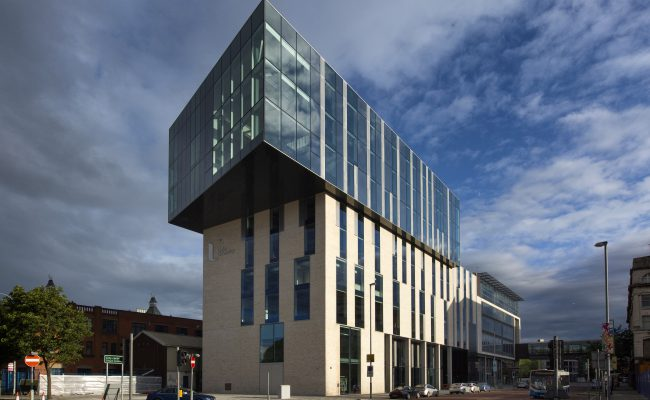
\includegraphics[width=0.4\textwidth, height=0.28\textwidth]{belfast_campus.jpg}
\end{center}
\vspace{-20pt}
  \caption{Introduction Banner.}
  \vspace{-0pt}
\end{wrapfigure}
%%%%%%%%%%%%%%%%%%%%%%
We propose exploring the problem of data augmentation for image and video classification, and evaluating different techniques.

\section{Related Work}
This section provides a brief review of past work that has augmented data to improve image classifier performance and the state of the art techniques of neural style transfer.
\subsection{Troditional Data Augmentation Tecniques}
Sed ut perspiciatis, unde omnis iste natus error sit voluptatem accusantium doloremque laudantium, totam rem aperiam eaque ipsa, quae ab illo inventore veritatis et quasi architecto beatae vitae dicta sunt, explicabo. Nemo enim ipsam voluptatem, quia voluptas sit, aspernatur aut odit aut fugit, sed quia consequuntur magni dolores eos, qui ratione voluptatem sequi nesciunt, neque porro quisquam est, qui dolorem ipsum, quia dolor sit amet consectetur adipisci[ng] velit, sed quia non numquam [do] eius modi tempora inci[di]dunt, ut labore et dolore magnam aliquam quaerat voluptatem. Ut enim ad minima veniam, quis nostrum exercitationem ullam corporis suscipit laboriosam, nisi ut aliquid ex ea commodi consequatur? Quis autem vel eum iure reprehenderit, qui in ea voluptate velit esse, quam nihil molestiae consequatur, vel illum, qui dolorem eum fugiat, quo voluptas nulla pariatur?

\subsubsection{Neural Style Transfer}
Sed ut perspiciatis, unde omnis iste natus error sit voluptatem accusantium doloremque laudantium, totam rem aperiam eaque ipsa, quae ab illo inventore veritatis et quasi architecto beatae vitae dicta sunt, explicabo. Nemo enim ipsam voluptatem, quia voluptas sit, aspernatur aut odit aut fugit, sed quia consequuntur magni dolores eos, qui ratione voluptatem sequi nesciunt, neque porro quisquam est, qui dolorem ipsum, quia dolor sit amet consectetur adipisci[ng] velit, sed quia non numquam [do] eius modi tempora inci[di]dunt, ut labore et dolore magnam aliquam quaerat voluptatem. Ut enim ad minima veniam, quis nostrum exercitationem ullam corporis suscipit laboriosam, nisi ut aliquid ex ea commodi consequatur? Quis autem vel eum iure reprehenderit, qui in ea voluptate velit esse, quam nihil molestiae consequatur, vel illum, qui dolorem eum fugiat, quo voluptas nulla pariatur?

%%
\section{Method}
Method. How to keep high level content. how to apply styles. the formulars.
\subsection{Datasets and Features} 
Sed ut perspiciatis, unde omnis iste natus error sit voluptatem accusantium doloremque laudantium, totam rem aperiam eaque ipsa, quae ab illo inventore veritatis et quasi architecto beatae vitae dicta sunt, explicabo. Nemo enim ipsam voluptatem, quia voluptas sit, aspernatur aut odit aut fugit, sed quia consequuntur magni dolores eos, qui ratione voluptatem sequi nesciunt, neque porro quisquam est, qui dolorem ipsum, quia dolor sit amet consectetur adipisci[ng] velit, sed quia non numquam [do] eius modi tempora inci[di]dunt, ut labore et dolore magnam aliquam quaerat voluptatem. Ut enim ad minima veniam, quis nostrum exercitationem ullam corporis suscipit laboriosam, nisi ut aliquid ex ea commodi consequatur? Quis autem vel eum iure reprehenderit, qui in ea voluptate velit esse, quam nihil molestiae consequatur, vel illum, qui dolorem eum fugiat, quo voluptas nulla pariatur?
\subsection{Baseline Network} 
Sed ut perspiciatis, unde omnis iste natus error sit voluptatem accusantium doloremque laudantium, totam rem aperiam eaque ipsa, quae ab illo inventore veritatis et quasi architecto beatae vitae dicta sunt, explicabo. Nemo enim ipsam voluptatem, quia voluptas sit, aspernatur aut odit aut fugit, sed quia consequuntur magni dolores eos, qui ratione voluptatem sequi nesciunt, neque porro quisquam est, qui dolorem ipsum, quia dolor sit amet consectetur adipisci[ng] velit, sed quia non numquam [do] eius modi tempora inci[di]dunt, ut labore et dolore magnam aliquam quaerat voluptatem. Ut enim ad minima veniam, quis nostrum exercitationem ullam corporis suscipit laboriosam, nisi ut aliquid ex ea commodi consequatur? Quis autem vel eum iure reprehenderit, qui in ea voluptate velit esse, quam nihil molestiae consequatur, vel illum, qui dolorem eum fugiat, quo voluptas nulla pariatur?


\section{Experiments}
Sed ut perspiciatis, unde omnis iste natus error sit voluptatem accusantium doloremque laudantium, totam rem aperiam eaque ipsa, quae ab illo inventore veritatis et quasi architecto beatae vitae dicta sunt, explicabo. Nemo enim ipsam voluptatem, quia voluptas sit, aspernatur aut odit aut fugit, sed quia consequuntur magni dolores eos, qui ratione voluptatem sequi nesciunt, neque porro quisquam est, qui dolorem ipsum, quia dolor sit amet consectetur adipisci[ng] velit, sed quia non numquam [do] eius modi tempora inci[di]dunt, ut labore et dolore magnam aliquam quaerat voluptatem. 
Consider the variable $x \in \mathbb{R}$, 
\begin{equation}
f(x)=x^2+2 \label{eq:mylabel}
\end{equation}
Equation (\ref{eq:mylabel}) is a polynomial of order 2.
%% comment line


\section{Result}
An example of table is shown Table \ref{tab:mytab}.
\begin{table}[!ht]
\begin{center}
\begin{tabular}{|c|c|c|}
\hline
x & y & z\\
\hline
\end{tabular}
\end{center}
\vspace{-20pt}
\caption{Example of table.} \label{tab:mytab}
  \vspace{-10pt}
\end{table}

\section{Conclusion}
The conclusion

\bibliographystyle{apalike}

\bibliography{imvip2018}


\end{document}

